% !TeX root = ../main.tex

\section{Resultate}

\begin{frame}{Resultate {\scriptsize \cite[S.~101-102]{stenningHumanReasoningCognitive2008}}}
    \begin{itemize}
        \item jede Manipulation bringt (unterschiedlich gute) Verbesserung
        \item entsprechend Vorhersagen der Theorien, von denen Manipulationen abgeleitet wurden
        \item starke Evidenz für Zusammenhang zwischen Manipulationen und mentalen Vorgängen, auf die sie einwirken
    \end{itemize}
\end{frame}


\begin{frame}{Resultate {\scriptsize \cite[S.~101]{stenningHumanReasoningCognitive2008}}}
    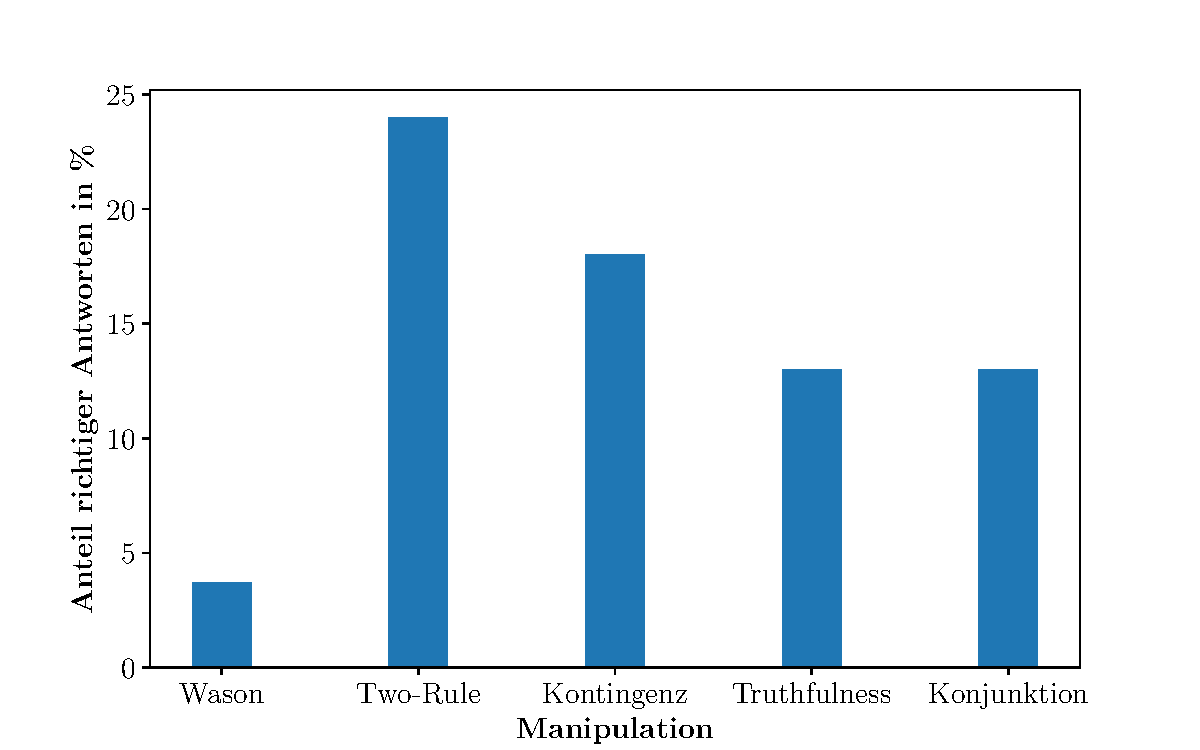
\includegraphics[width=\textwidth]{../plot/results_correct.pdf}
\end{frame}


\begin{frame}{Two-Rule Task {\scriptsize \cite[S.~102-104]{stenningHumanReasoningCognitive2008}}}
    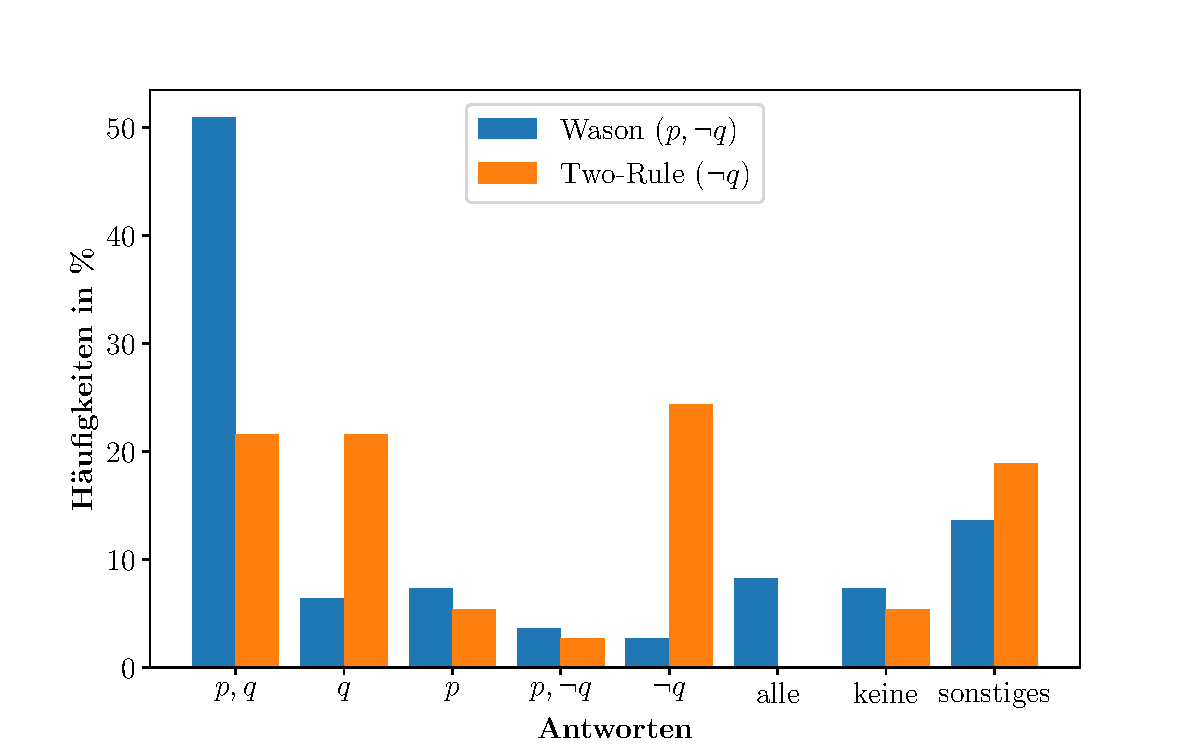
\includegraphics[width=\textwidth]{../plot/results_two_rule.pdf}
\end{frame}


\begin{frame}{Two-Rule Task {\scriptsize \cite[S.~102-104]{stenningHumanReasoningCognitive2008}}}
    $(p \to q) \leadsto (\{U, I\} \to 8)$

    \begin{itemize}
        \item Verwechslungsgefahr zwischen
        \begin{itemize}
            \item \enquote{diese Regel trifft auf diese Karte zu}
            \item \enquote{diese Karte macht diese Regel wahr}
        \end{itemize}
        
        \item $q~\hat=~8$ könnte beide Regeln bestätigen \\
            $\Rightarrow$ Konflikt: eine Regel wahr, eine falsch
        
        \item asymmetrische Beziehung von \emph{true}
        
        \item Information-Gain: $\lnot q$ bietet am meisten Informationen \\
            $\Rightarrow$ Vorhersage: häufigste Wahl
        \begin{itemize}
            % Achtung: hier Widerspruch!
            % Buch schreibt "false-consequent card comes in third"
            % Daten in Tabelle 4.2 und 4.4
            \item Beobachtung: tatsächlich häufigste Antwort
        \end{itemize}
    \end{itemize}
\end{frame}



\begin{frame}{Kontingenz {\scriptsize \cite[S.~109]{stenningHumanReasoningCognitive2008}}}
    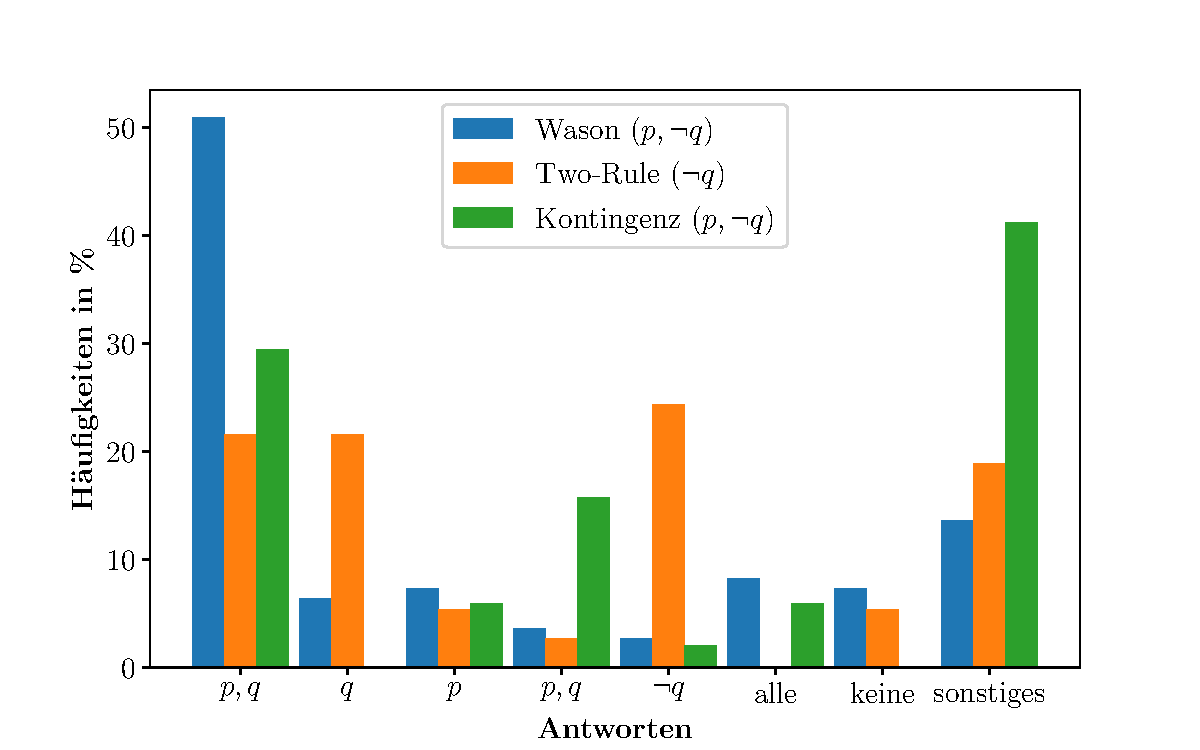
\includegraphics[width=\textwidth]{../plot/results_contingency.pdf}
\end{frame}


\begin{frame}{Truthfulness {\scriptsize \cite[S.~109]{stenningHumanReasoningCognitive2008}}}
    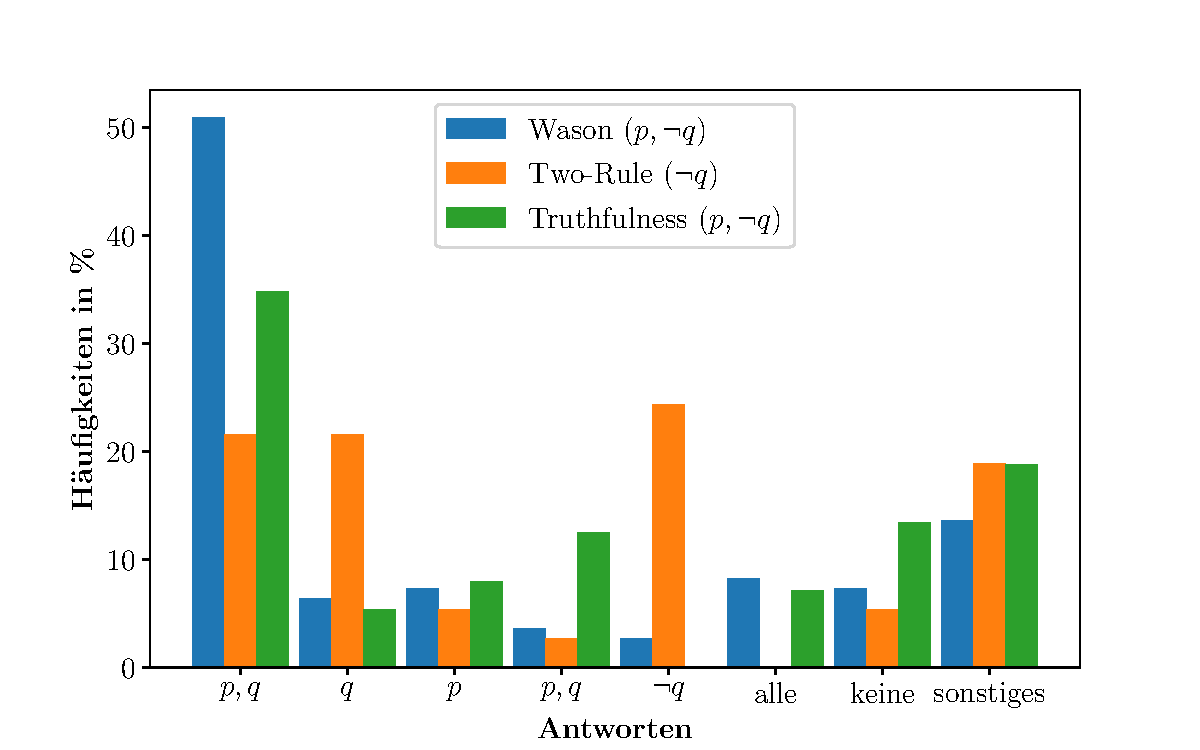
\includegraphics[width=\textwidth]{../plot/results_truthfulness.pdf}
\end{frame}


\begin{frame}{Konjunktion {\scriptsize \cite[S.~109]{stenningHumanReasoningCognitive2008}}}
    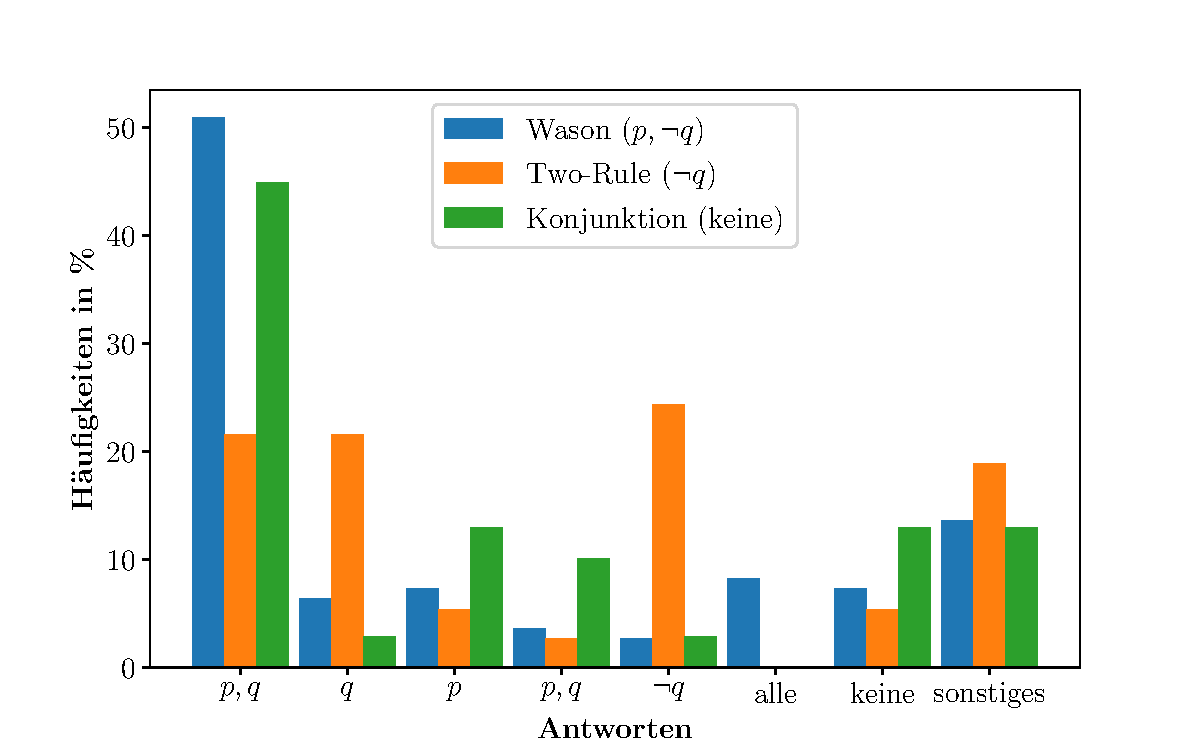
\includegraphics[width=\textwidth]{../plot/results_conjunction.pdf}
\end{frame}


\begin{frame}{Konjunktivisch {\scriptsize \cite[S.~109]{stenningHumanReasoningCognitive2008}}}
    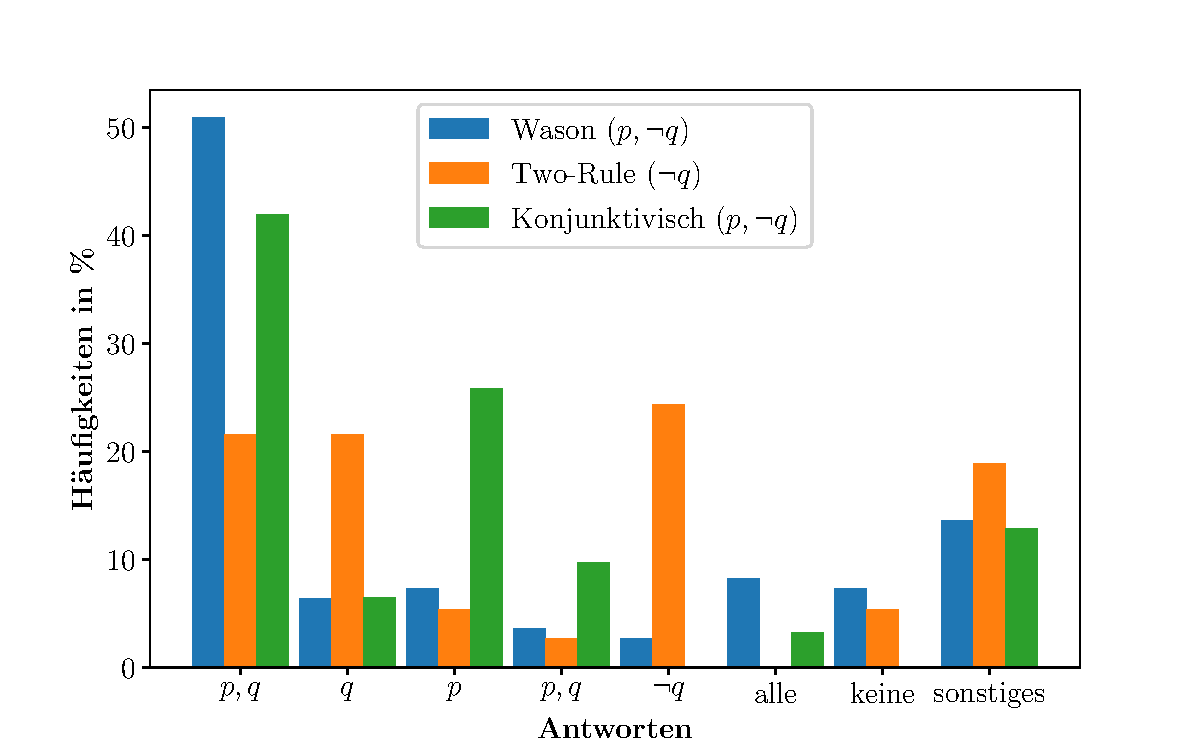
\includegraphics[width=\textwidth]{../plot/results_subjunctive.pdf}
\end{frame}
